\documentclass[12pt]{article}

%useful packages
\usepackage{color,soul}
\usepackage[usenames,dvipsnames,svgnames,table]{xcolor}
\usepackage{amsmath,amsthm,amscd,amssymb,bm}
\usepackage{hyperref}
\hypersetup{
    colorlinks=true,
    linkcolor=JungleGreen,
    urlcolor  =JungleGreen,
    citecolor = JungleGreen,
    anchorcolor = JungleGreen
}
\usepackage[utf8]{inputenc}
\usepackage[top=2cm, bottom=3cm, left=2cm, right=2cm]{geometry}
\usepackage{pgfplots}
\usepackage{enumitem}
\usepgfplotslibrary{fillbetween}
\usetikzlibrary{patterns}
\usepackage{tcolorbox}
\usepackage{centernot}
\usepackage{mathtools}
\usepackage{xcolor}
\usepackage{subcaption}

%personal definitions and commands
\newcommand{\R}{\mathbb{R}} 
\newcommand{\E}{\mathbb{E}}
\newcommand{\V}{\mathbb{V}}
\newcommand{\C}{\mathbb{C}}
\newcommand{\Prob}{\mathbb{P}}
\newcommand{\e}{\epsilon}
\newcommand\numberthis{\addtocounter{equation}{1}\tag{\theequation}} %allows numbering of single equations in align* environment
\newcommand{\mtx}[1]{\ensuremath{\bm{\mathit{#1}}}}
\newcommand{\B}{\hat{\boldsymbol{\beta}}}
\newcommand{\Cov}{\mathbb{C}\text{ov}}
\newcommand{\N}{\mathcal{N}}



\title{ECON675 -- Assignment 6}
\author{Anirudh Yadav}
\setlength\parindent{0pt}
\begin{document}

\maketitle

\setcounter{tocdepth}{2}
\tableofcontents

\newpage

\section{Continuity-based identification in SRD designs}

\subsection{RD treatment effect with a single cutoff}
We have
\begin{align*}
\tau_{\texttt{SRD}} = \lim_{\e \to 0^+} \E[Y_i | \tilde{X}_i = \e] - \lim_{\e \to 0^+} \E[Y_i | \tilde{X}_i = -\e]
\end{align*}
Using the definition $\tilde X_i = X_i - C_i$ and the single cutoff assumption, $\Prob[C_i = c] = 1$, gives
\begin{align*}
\tau_{\texttt{SRD}} &= \lim_{\e \to 0^+} \E[Y_i | X_i= c+ \e] - \lim_{\e \to 0^+} \E[Y_i | X_i = c -\e]\\
&= \lim_{\e \to 0^+} \E[Y_{1i}(c)T_i + Y_{0i}(c)(1-T_i)| X_i= c+ \e] - \lim_{\e \to 0^+} \E[Y_{1i}(c)T_i + Y_{0i}(c)(1-T_i) | X_i = c -\e]\\
&= \lim_{\e \to 0^+} \E[Y_{1i}(c)| X_i= c+ \e] - \lim_{\e \to 0^+} \E[Y_{0i}(c)| X_i = c -\e], \text{ using \textbf{S3}}\\
&= \E[Y_{1i}(c)-Y_{0i}(c)| X_i= c],
\end{align*}
as required.

\subsection{RD treatment effect with multiple cutoffs}
Now, with multiple cutoffs
\begin{align*}
\tau_{\texttt{SRD}} &= \lim_{\e \to 0^+} \E[Y_i | \tilde{X}_i = \e] - \lim_{\e \to 0^+} \E[Y_i | \tilde{X}_i = -\e]\\
\end{align*}
Focusing on the first term on the RHS:
\begin{align*}
 \lim_{\e \to 0^+} \E[Y_i | \tilde{X}_i = \e]  &=   \lim_{\e \to 0^+} \E[Y_{1i}(C_i)T_i + Y_{0i}(C_i)(1-T_i)| X_i= C_i+ \e]\\
 &=\E[Y_{1i}(C_i)| X_i= C_i] \text{ using \textbf{S3}},\\
 &=\sum_{c\in \mathcal{C}}\E[Y_{1i}(C_i)| X_i=c, C_i = c]\Prob[X_i=c, C_i=c], \text{ since $C_i$ is a discrete r.v},\\
 &=\sum_{c\in \mathcal{C}}\E[Y_{1i}(C_i)| X_i=c, C_i = c] \frac{f_{X|C}(c|c)\Prob[C_i=c]}{\sum_{c\in \mathcal{C}}f_{X|C}(c|c)\Prob[C_i=c]}.
\end{align*}
An analogous derivation shows that $$\lim_{\e \to 0^+} \E[Y_i | \tilde{X}_i = -\e] = \sum_{c\in \mathcal{C}}\E[Y_{0i}(C_i)| X_i=c, C_i = c] \frac{f_{X|C}(c|c)\Prob[C_i=c]}{\sum_{c\in \mathcal{C}}f_{X|C}(c|c)\Prob[C_i=c]},$$ which proves the desired result. In this case, $\tau_{\texttt{SRD}}$ is just a weighted average of the RD treatment effects for the different cutoff levels. 

\subsection{RD treatment effect with individual heterogeneity}
First consider the case with a single cutoff, $\Prob[C_i=c]=1$. Suppose that $W_i$ is a continuous random variable, with marginal cdf $G(\cdot)$, that affects $i$'s potential outcomes and is iid across observations. Now,
\begin{align*}
\tau_{\texttt{SRD}} &= \lim_{\e \to 0^+} \E[y_{1}(w_i) | X_i=c+ \e] - \lim_{\e \to 0^+} \E[y_{0}(w_i)| X_i = c -\e]\\
&=\E[y_{1}(w_i) - y_{0}(w_i) | X_i=c]\\
&= \int (y_{1}(w) - y_{0}(w))g_{W|X}(w)|_{X=c}
\end{align*}
Now, using Bayes' rule
\begin{align*}
g_{W|X}(w) = \frac{f(X|W)g(w)}{f(X)}
\end{align*}
where $f(\cdot)$ is the marginal density of the running variable $X_i$. Thus, for the single cutoff case
\begin{align*}
\tau_{\texttt{SRD}} &= \int (y_{1}(w) - y_{0}(w)) \frac{f_{X|W}(c)}{f(c)}g(w)dw
\end{align*}
which is the result presented by Lee (2008). Then, you can extend the multiple cutoff case to get the desired result.

\newpage

\section{The effect of Head Start on child mortality}

\subsection{RD plots and falsification tests}
\begin{figure}[htpb!]
    \centering
    \caption{RD Plots of Pre-intervention Mortality Rates Using Different Binning Procedures}
    \begin{minipage}{0.5\textwidth}
        %\centering
        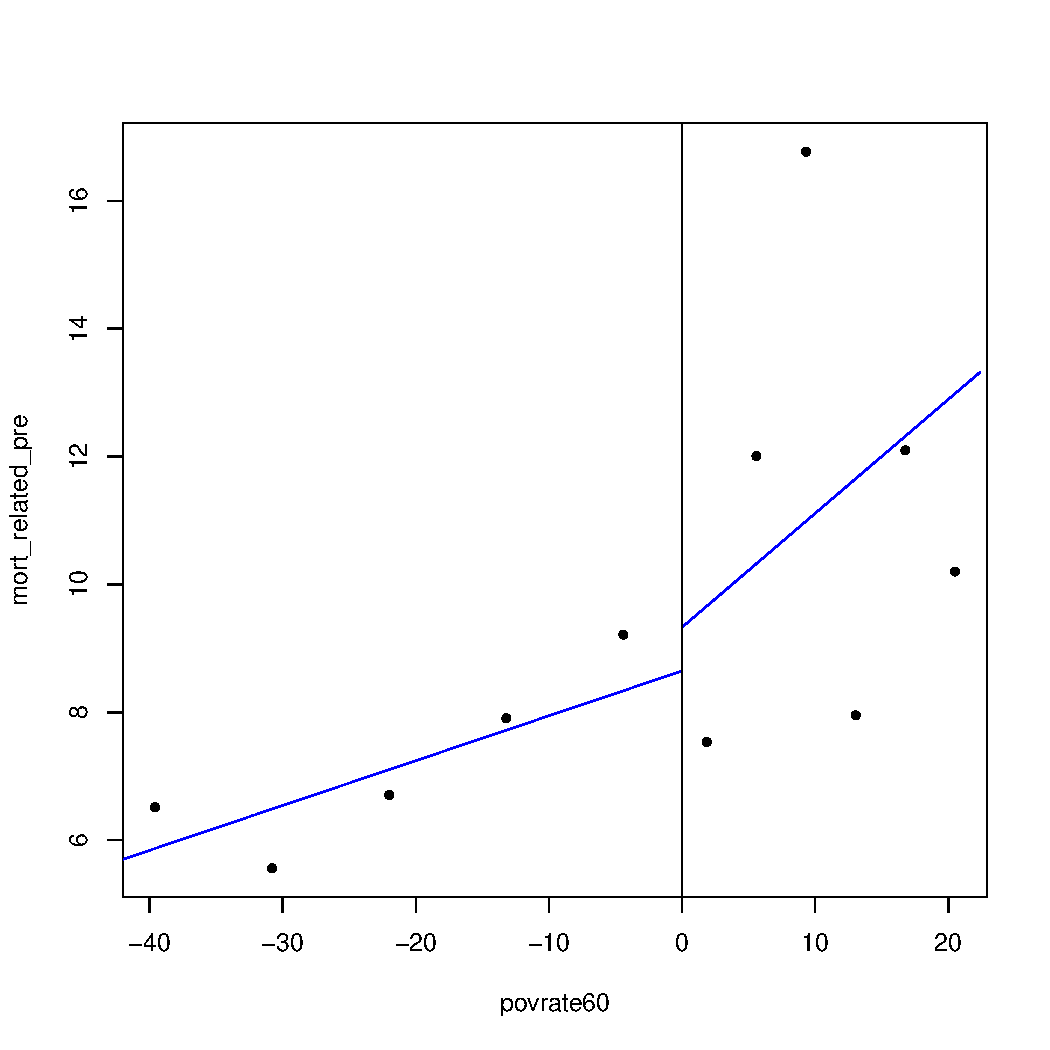
\includegraphics[width=1\textwidth]{q2-1-es.pdf}
        \subcaption{Evenly-spaced, IMSE optimal}
    \end{minipage}\hfill
    \begin{minipage}{0.5\textwidth}
      %  \centering
        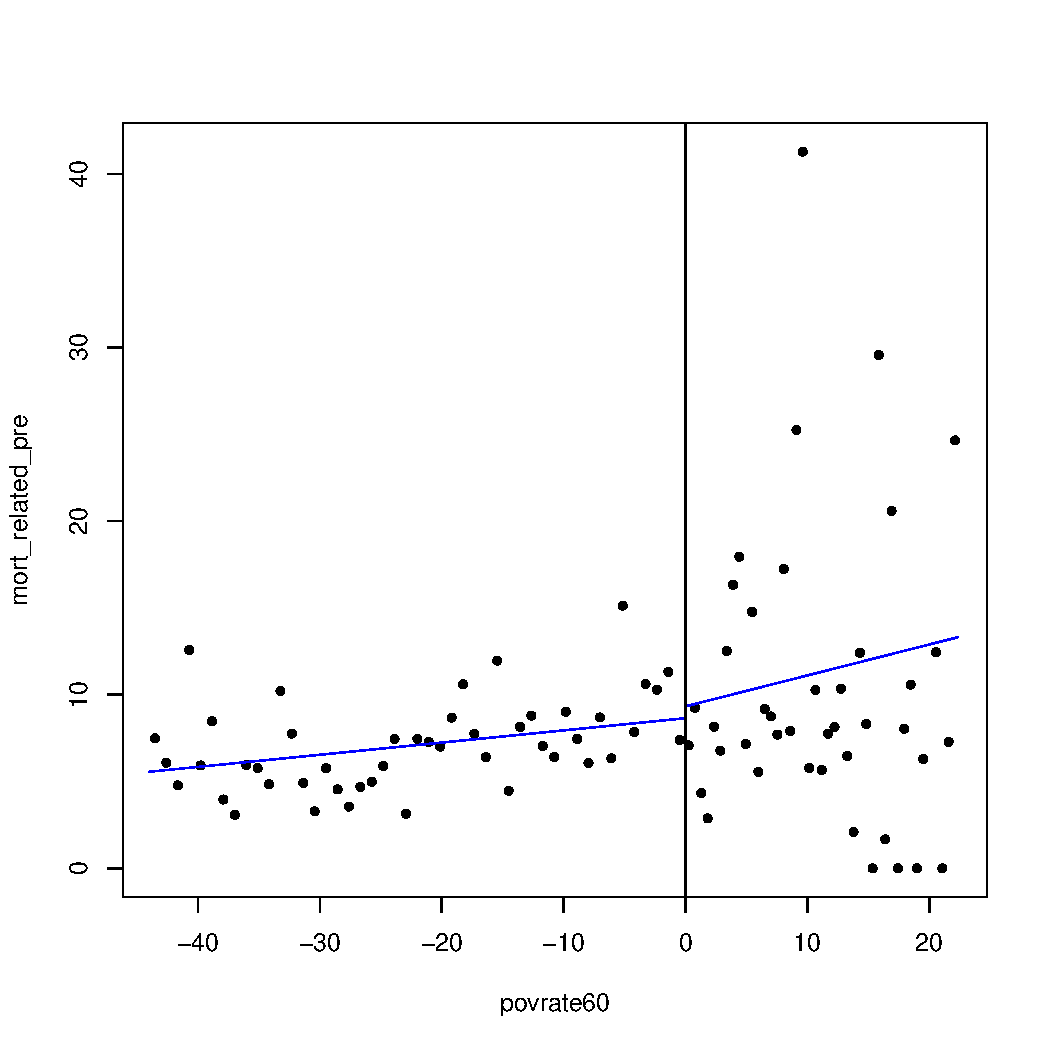
\includegraphics[width=1\textwidth]{q2-1-esmv.pdf}
        \subcaption{Evenly-spaced, variance mimicking}
    \end{minipage}
\centering
\begin{minipage}{0.5\textwidth}
        %\centering
        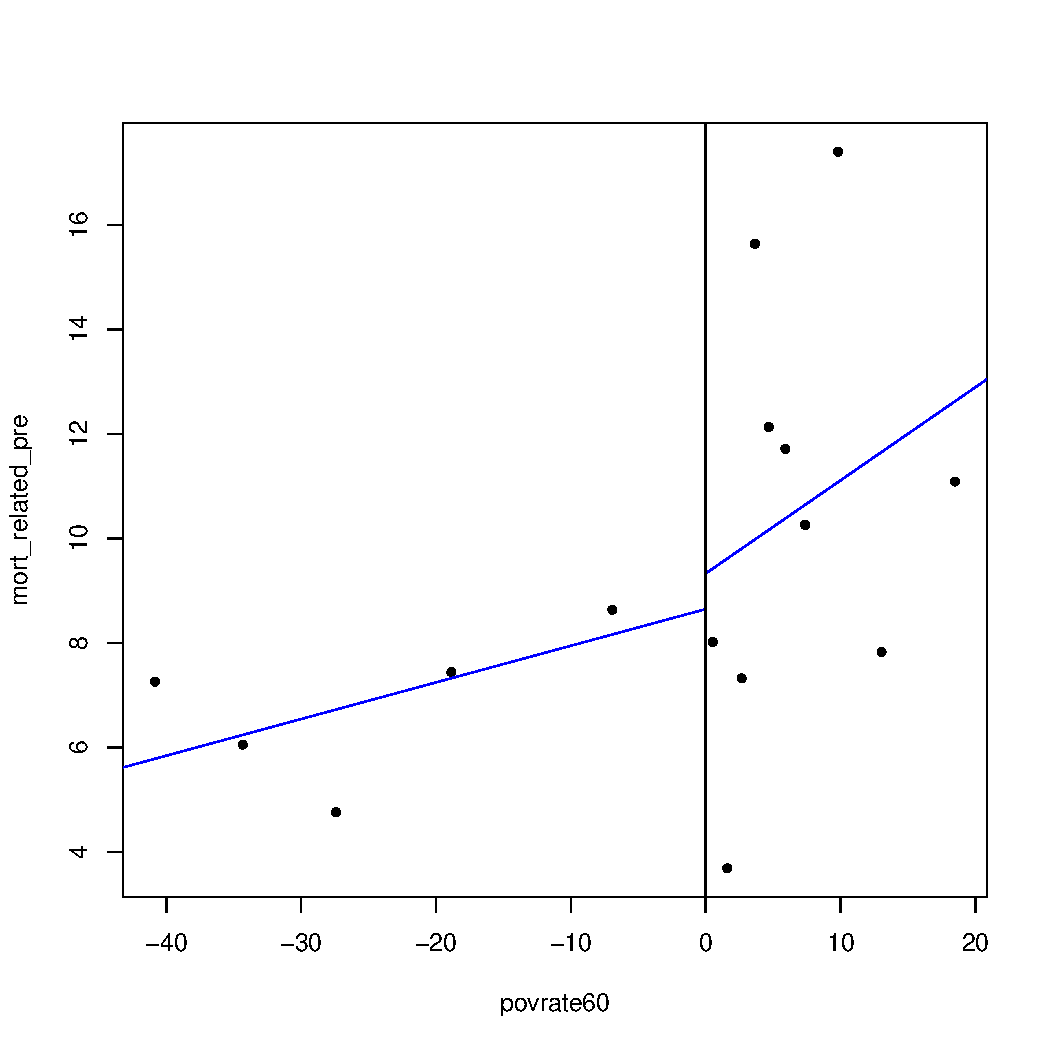
\includegraphics[width=1\textwidth]{q2-1-qs.pdf}
        \subcaption{Quantile-spaced, IMSE optimal}
    \end{minipage}\hfill
    \begin{minipage}{0.5\textwidth}
      %  \centering
        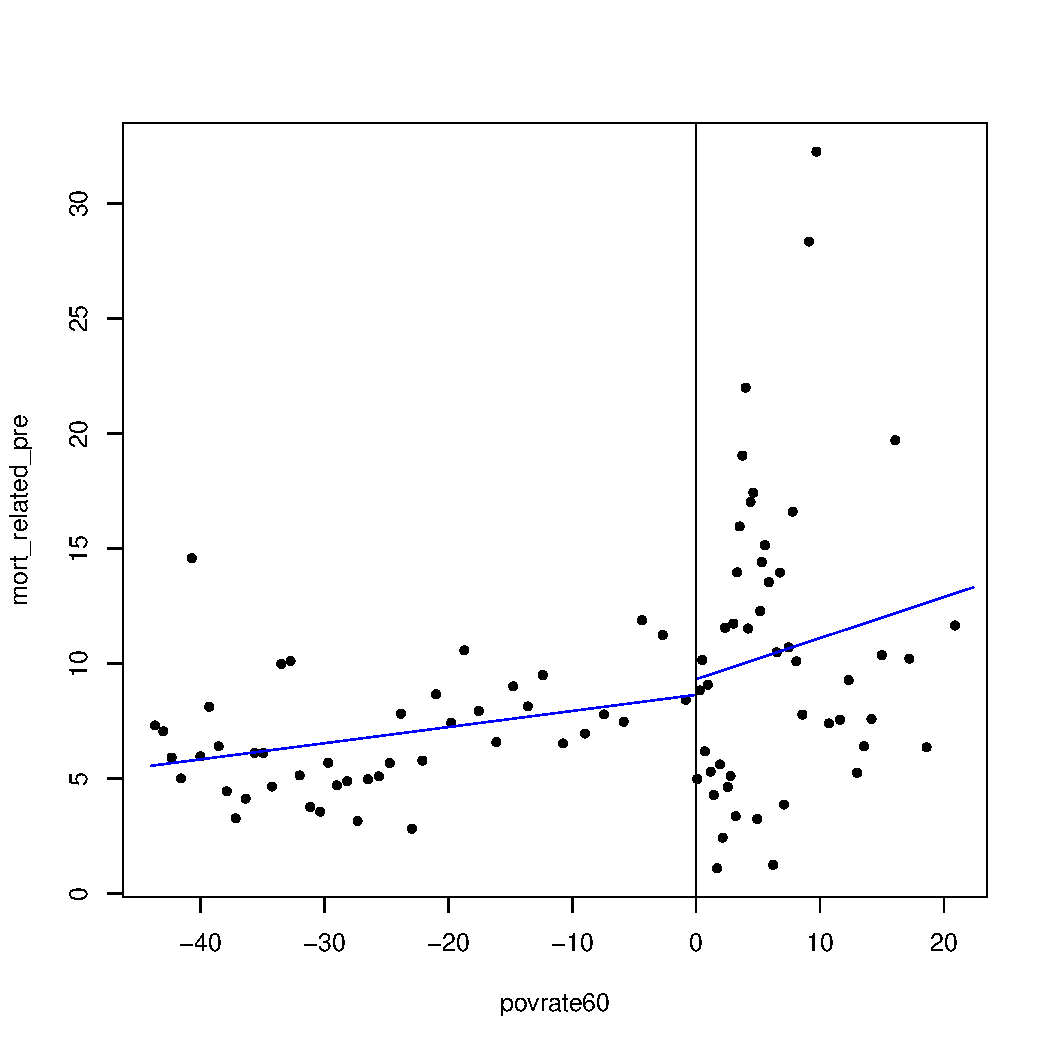
\includegraphics[width=1\textwidth]{q2-1-qsmv.pdf}
        \subcaption{Quantile-spaced, variance mimicking}
    \end{minipage}
\end{figure}

Figure 1 shows the RD plots of \verb|mort_related_pre| using different binning procedures, as required. For each binning method, there is clearly no evidence of a negative discontinuity at the cutoff poverty rate. (In fact, there seems to be a small positive jump in pre-invervention mortality rates at the cutoff.) If there was a negative jump in pre-intervention mortality rates at the cutoff this would potentially falsify the proposed RD design because it would provide strong evidence that the counties assigned to Head Start treatment had systematically lower mortality rates prior to the intervention.\\

We can also conduct formal falsification tests. First, I conduct exact binomial tests for small windows around the cutoff. The basic idea is that if there is no systematic sorting, then the number of observations just above or below the cutoff should be pretty close to random, and thus should follow a binomial distribution. Table 1 shows the results for the exact binomial test (with probability of success set to 0.5) for a few small windows near the cutoff (replicating Table 1 in Cattaneo, \textit{et al}. (2017)). Clearly, we cannot reject the null that the number of observations just above and below the cutoff are random.

\begin{table}[htpb!]
\centering
\caption{Binomial tests}
\begin{tabular}{llrrr}
  \hline
 & $h$ & $N_W^-$ & $N_W^+$ & $p$-value \\ 
  \hline
1 & 0.3 & 9 & 10 & 1.000 \\ 
  2 & 0.5 & 18 & 16 & 0.864 \\ 
  3 & 0.7 & 24 & 22 & 0.883 \\ 
  4 & 0.9 & 32 & 27 & 0.603 \\ 
  5 & 1.1 & 43 & 33 & 0.302 \\ 
  6 & 1.3 & 51 & 38 & 0.203 \\ 
   \hline
\end{tabular}
\end{table}

Next, I test for a discontinuity in the density of the running variable at the cutoff, as in Cattaneo, \textit{et al}. (2017), using the \verb|rddensity| package in \verb|R|. I compute the density test $p$-value using the package defaults, which specifies a local-quadratic polynomial estimator with triangular kernel and jackknife standard errors. I get $p = 0.639$, implying that we cannot reject the null that the density of the running variable is continuous at the cutoff.

\subsection{Global and flexible parametric methods -- BAD!}
\subsubsection{Constant treatment effect}
I estimate the following global polynomial regression models
\begin{align*}
y_i = \alpha_0 + \tau_{\texttt{SRD}} t_i + \sum_{k=1}^p \beta_k x_i^k + \e_i
\end{align*}
where $y_i$ is the outcome of interest (post-intervention mortality rate) and $x_i$ is the running variable (poverty rate in 1960) and $t_i$ is a treatment dummy equal to 1 if $x_i \geq 0$. Table 2 presents the point estimates of $\tau_{\texttt{SRD}}$ for $p=3,4,5,6$ and the corresponding robust standard errors. The estimated treatment effects are all negative as expected. I also plot the fitted values for $p=4$ below.

\begin{table}[htpb!]
\centering
\caption{Global Polynomial Fit under Constant Treatment Effect Assumption}
\begin{tabular}{lrrrr}
  \hline
 & $p=3$ & $p=4$ & $p=5$ & $p=6$ \\ 
  \hline
Point estimate& $-1.12$ & $-1.02$ & $-1.66$ & $-1.75$ \\ 
Std. err. & 0.59 & 0.75 & 0.81 & 0.86 \\ 
   \hline
\end{tabular}
\end{table}
\captionsetup[figure]{font=small,skip=0pt}

\begin{figure}[htpb!]
    \centering
    \caption{Fitted Values for 4-th Order Global Polynomial -- Constant Effect Assumption}
        %\centering
        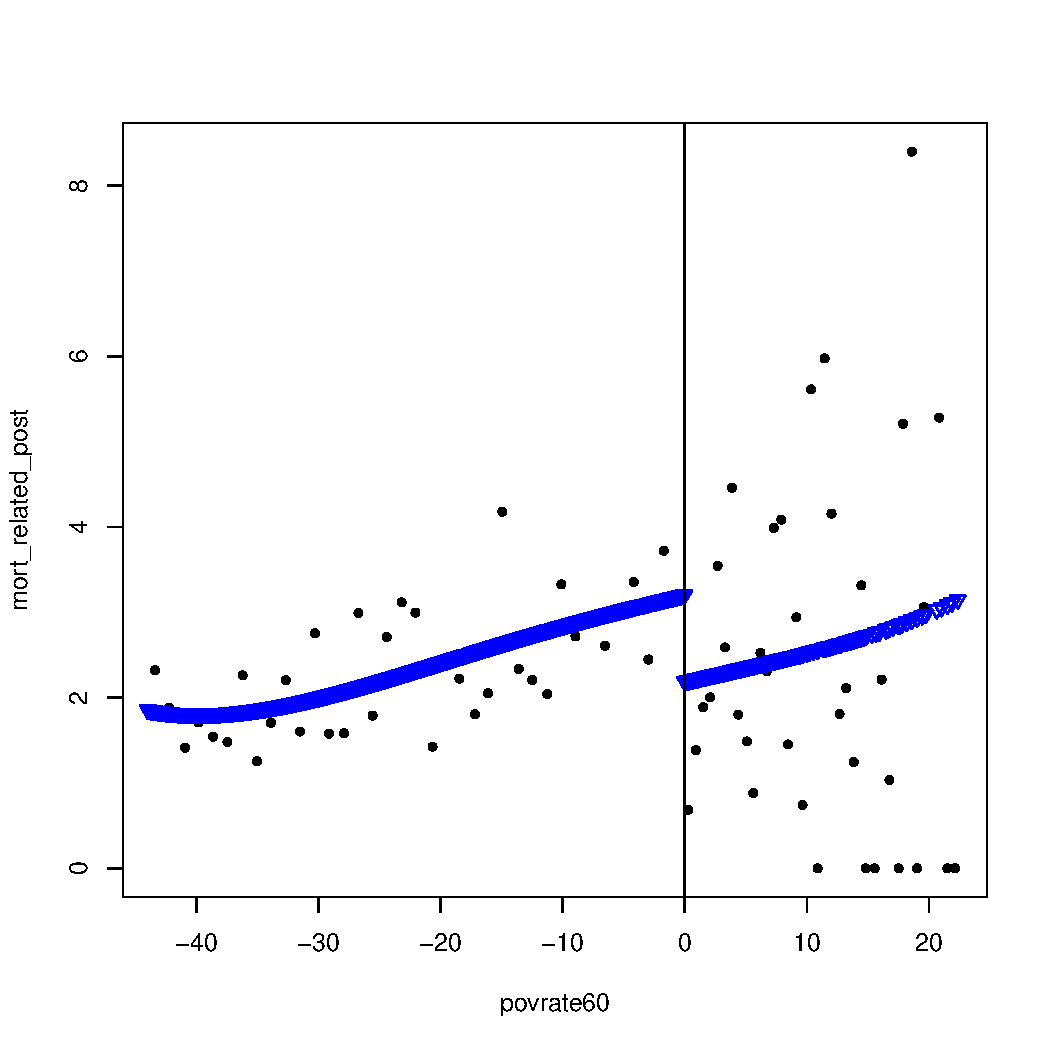
\includegraphics[width=0.7\textwidth]{q2-2-const.pdf}
\end{figure}

\subsubsection{Fully interacted model}
Next, I estimate the `fully-interacted' models
\begin{align*}
y_i = \alpha_0 +\tau_{\texttt{SRD}} t_i + \sum_{k=1}^p \beta_k t_i x_i^k + \e_i.
\end{align*}
These models amount to fitting a global polynomial of order $p$ separately on both sides of the cutoff. Table 3 shows the point estimates of $\tau_{\texttt{SRD}}$ for $p=3,4,5,6$ and the corresponding robust standard errors.

\begin{table}[htpb!]
\centering
\caption{Global Polynomial Fit Separately on Both Sides of the Cutoff}
\begin{tabular}{lrrrr}
  \hline
 & $p=3$ & $p=4$ & $p=5$ & $p=6$ \\  
  \hline
Point estimate & $-2.02$ & $-3.06$ & $-2.68$ & $-4.12$ \\ 
Std. err. & 0.87 & 1.09 & 1.29 & 1.46 \\ 
   \hline
\end{tabular}
\end{table}


\begin{figure}[htpb!]
    \centering
    \caption{Fitted Values for 4-th Order Global Polynomial -- Fully Interacted Model}
        %\centering
        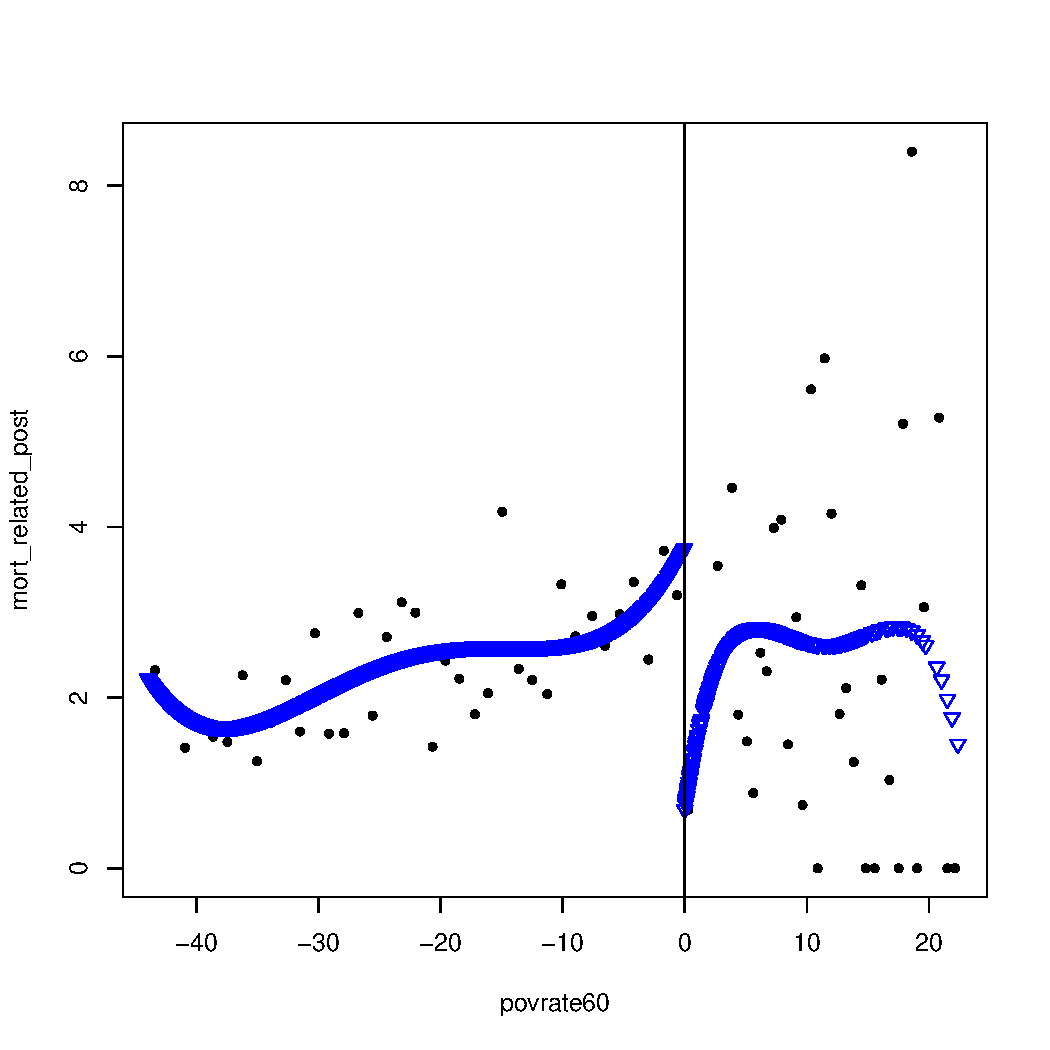
\includegraphics[width=0.7\textwidth]{q2-2-full.pdf}
\end{figure}

Despite the negative estimated treatment effects, these are bad models. They all use global methods, but we know that RD treatment effects are inherently local to the cutoff. In essence, global methods do not compare `apples with apples', because counties well below or above the cutoff could be different in systematically important ways.

\subsection{Robust local polynomial methods}

\subsubsection{Baseline estimates}
Table 4 shows the MSE-optimal RD point estimators and robust confidence intervals using local constant, linear and quadratic estimators (implemented with the \verb|rdrobust| package in \verb|R|). The estimated treatment effects are negative and significantly different from zero for all specifications, as expected. The standard errors of the point estimates increase with the order of the local polynomial.

\begin{table}[htpb!]
\centering
\caption{MSE-Optimal RD Treatment Effects with Different Polynomial Estimators}
\begin{tabular}{lrrrr}
  \hline
 & Coeff & Std. Err. & CI Lower & CI Upper \\ 
  \hline
  \multicolumn{5}{c}{$p=0$}\\
  \hline
Conventional & -2.11 & 0.99 & -4.05 & -0.17 \\ 
  Bias-Corrected & -2.56 & 0.99 & -4.50 & -0.62 \\ 
  Robust & -2.56 & 1.23 & -4.96 & -0.15 \\ 
   \hline
   \multicolumn{5}{c}{$p=1$}\\
     \hline
Conventional & -2.41 & 1.21 & -4.77 & -0.05 \\ 
  Bias-Corrected & -2.78 & 1.21 & -5.14 & -0.42 \\ 
  Robust & -2.78 & 1.37 & -5.46 & -0.10 \\ 
   \hline
\multicolumn{5}{c}{$p=2$}\\
     \hline
Conventional & -3.47 & 1.37 & -6.16 & -0.79 \\ 
  Bias-Corrected & -3.78 & 1.37 & -6.46 & -1.10 \\ 
  Robust & -3.78 & 1.45 & -6.62 & -0.94 \\ 
   \hline
\end{tabular}
\end{table}

\subsubsection{Placebo tests}
Table 5 shows estimated RD treatment effects for the pre-intervention outcome variable \verb|mort_related_pre| and the unaffected post-intervention variable, \verb|mort_injury_post|. Clearly, we cannot reject the null of no treatment effect on these placebo outcomes.

\begin{table}[htpb!]
\centering
\caption{Robustness Checks of RD Treatment Effects using Different Outcome Variables}
\begin{tabular}{lrrrr}
  \hline
 & Coeff & Std. Err. & CI Lower & CI Upper \\ 
  \hline
  \multicolumn{5}{c}{$y= \texttt{mort\_related\_pre}$}\\
  \hline
Conventional & -2.38 & 2.25 & -6.78 & 2.03 \\ 
  Bias-Corrected & -1.77 & 2.25 & -6.17 & 2.64 \\ 
  Robust & -1.77 & 2.68 & -7.01 & 3.48 \\ 
   \hline
 \multicolumn{5}{c}{$y= \texttt{mort\_injury\_post}$}\\
     \hline
Conventional & 1.13 & 3.77 & -6.26 & 8.53 \\ 
  Bias-Corrected & 1.52 & 3.77 & -5.87 & 8.92 \\ 
  Robust & 1.52 & 4.39 & -7.07 & 10.12 \\
   \hline
\end{tabular}
\end{table}

\subsubsection{Donut holes!}
Table 6 shows the point estimates for the `donut hole' robustness checks, where I drop the $\ell$ closest observations on either side of the cuttoff.
\begin{table}[htpb!]
\centering
\caption{Donut Hole Robustness Check}
\begin{tabular}{lrrrrrrrrrr}
  \hline
 \# obs. dropped ($\ell$) & 1 & 2 & 3 & 4 & 5 & 6 & 7 & 8 & 9 & 10 \\ 
  \hline
Point estimate& -2.80 & -2.83 & -2.93 & -2.62 & -2.65 & -2.28 & -2.33 & -2.86 & -2.38 & -2.44 \\ 
   \hline
\end{tabular}
\end{table}

\subsubsection{Placebo cutoffs}
Self explanatory.
\begin{table}[htpb!]
\centering
\caption{Placebo Cutoffs Robustness Check}
\begin{tabular}{lrrrrrrrrrrr}
  \hline
 $c$ & -10 & -8 & -6 & -4 & -2 & 0 & 2 & 4 & 6 & 8 & 10 \\   
 \hline
 
  Point estimate & 0.55 & -0.26 & 0.40 & -0.09 & 2.24 & -2.78 & 3.13 & -1.53 & 1.64 & -5.80 & 4.18 \\ 
  $p$-val. & 0.56 & 0.82 & 0.70 & 0.94 & 0.24 & 0.04 & 0.04 & 0.38 & 0.19 & 0.10 & 0.37 \\ 
   \hline
\end{tabular}
\end{table}

\subsection{Local randomization inference}
I use the \verb|rdlocrand| package in \verb|R| to conduct local randomization inference on the Head Start data.

\subsubsection{Window selection}
First we need to select a window around the cutoff where randomization inference is appropriate. To do so, I use the \verb|rdwinselect| function in \verb|R|, with pre-intervention covariate \verb|mort_related_pre| and the unaffected post-intervention variable, \verb|mort_injury_post|. The basic idea is to choose the largest window around the cutoff where these covariates (which should not be related to the treatment) are ``reasonably'' balanced for counties above and below the cutoff. Essentially, we're trying to choose the biggest window around the cutoff where counties' poverty rates are pretty much random. Within this window, the RD design can be interpreted as a randomized experiment.\\

Using \verb|rdwinselect| (and the default options), the recommended window is $[-0.976;0.976]$ with 126 observations (68 below, 58 above).

\subsubsection{Fisher's approach}
With the recommended window above, the observed difference in means is $-2.304\%$, with Fisher $p$-value of $0.024$ (associated with the sharp null of no treatment effect and 1000 replications).

\subsubsection{Neyman's approach}
For Neyman's approach, I compute the difference in means between the treatment and control groups, for different windows around the cutoff. To implement this approach I simply run the simple linear regression
\begin{align*}
y_i = \alpha_0 + \beta_0t_i + \e_i.
\end{align*}
where $t_i$ is a treatment dummy equal to 1 if county $i$'s poverty rate is above the cutoff. The point estimate $\hat{\beta}_0$ gives me the difference in sample means.

\begin{table}[htpb!]
\centering
\begin{tabular}{lrrrrrrrrrr}
  \hline
$w$ & 0.80 & 1.00 & 1.20 & 1.40 & 1.60 & 1.80 & 2.00 & 2.20 & 2.40 & 2.60 \\ 
  \hline
  $\hat{\beta}_0$& -1.66 & -2.31 & -2.19 & -3.09 & -2.94 & -2.56 & -2.52 & -2.47 & -2.00 & -1.76 \\ 
  Robust std. err. & 0.99 & 0.90 & 0.82 & 1.38 & 1.36 & 1.20 & 1.10 & 1.05 & 1.04 & 1.00 \\ 
  $p$-val. & 0.10 & 0.01 & 0.01 & 0.03 & 0.03 & 0.04 & 0.02 & 0.02 & 0.06 & 0.08 \\ 
   \hline
\end{tabular}
\end{table}

\newpage


\section{Appendix: \texttt{R} code}

\scriptsize
\begin{verbatim}
## ECON675: ASSIGNMENT 6
## Q2: THE EFFECT OF HEAD START ON CHILD MORTALITY
## Anirudh Yadav 
## 12/07/2018

######################################################################
# Load packages, clear workspace
######################################################################
rm(list = ls())             #clear workspace
library(foreach)            #for looping
library(data.table)         #for data manipulation
library(Matrix)             #fast matrix calcs
library(ggplot2)            #for pretty plots
library(sandwich)           #for variance-covariance estimation 
library(xtable)             #for latex tables
library(rdrobust)           #for RD plots and other stuff
library(rddensity)          #for RD density continuity tests
library(rdlocrand)          #for RD randomization inference
options(scipen = 999)       #forces R to use normal numbers instead of scientific notation

######################################################################
# Input data
######################################################################
setwd("/Users/Anirudh/Desktop/GitHub/PhD_Coursework/ECON675/HW6")
data <- as.data.table(read.csv('HeadStart.csv'))

######################################################################
# [2.1]A RD Plots of pre-intervention mortality
######################################################################

# Evenly-spaced bins, IMSE optimal
rdplot(data[,mort_related_pre],data[,povrate60],p=1,binselect = "es",x.label="povrate60",y.label="mort_related_pre",title="")
dev.copy(pdf,'q2-1-es.pdf')
dev.off()

# Evenly-spaced bins, mimicking variance 
rdplot(data[,mort_related_pre],data[,povrate60],p=1,binselect = "esmv",x.label="povrate60",y.label="mort_related_pre",title="")
dev.copy(pdf,'q2-1-esmv.pdf')
dev.off()

# Quantile-spaced bins, IMSE optimal
rdplot(data[,mort_related_pre],data[,povrate60],p=1,binselect = "qs",x.label="povrate60",y.label="mort_related_pre",title="")
dev.copy(pdf,'q2-1-qs.pdf')
dev.off()

# Quantile-spaced bins, mimicking variance
rdplot(data[,mort_related_pre],data[,povrate60],p=1,binselect = "qsmv",x.label="povrate60",y.label="mort_related_pre",title="")
dev.copy(pdf,'q2-1-qsmv.pdf')
dev.off()

######################################################################
# [2.1]B Formal falsification tests
######################################################################

## Exact binomial tests for different windows around the cutoff

# Vector of windows
h.vec = seq(0.3,1.3,0.2)

# Get running variable
x     = data[,povrate60]

# Number of observations just above and below the cutoff
N.l   = sapply(1:length(h.vec),function(i) sum(x >= -h.vec[i] & x <=0))
N.u   = sapply(1:length(h.vec),function(i) sum(x >= 0 & x <= h.vec[i]))

# Total number of observations in the window
N.t   = N.l + N.u

# Conduct exact binomial tests (p=0.5), where success is treatment and store p-vals
binom.pvals = sapply(1:length(h.vec),function(i) binom.test(N.u[i],N.t[i])$p.value)

# Put results together for latex
binom.results = cbind(h.vec,N.l,N.u,binom.pvals)
xtable(binom.results,digits = c(0,1,0,0,3))

## Continuity in density tests (defaults are triangular kernel, jackknife SEs)
rdtest = rddensity(x)

######################################################################
# [2.2]A Global polynomial regression - constant treatment effect
######################################################################

# Create treatment dummy for regressions
treat=ifelse(data[,povrate60]>=0,1,0)

# Get outcome variable
Y = data[,mort_related_post]

# Generate covariates for polynomial regressions
X.pol = cbind(x,x^2,x^3,x^4,x^5,x^6)

# Run polynomial regressions
global.regs = lapply(0:3,function(i) lm(Y ~ treat + X.pol[,c(1:(3+i))]))

# Get point estimates
global.betas = sapply(1:4,function(i) global.regs[[i]]$coefficients[2])

# Get robust SEs
global.SEs   = sapply(1:4,function(i) sqrt(diag(vcovHC(global.regs[[i]],"HC2")))[2])

# Put results together
global.results = rbind(global.betas, global.SEs)
colnames(global.results) = c(3,4,5,6)
xtable(global.results,digits=c(0,2,2,2,2))

# Plot fitted values and data
temp.rd = rdplot(Y,x,hide=TRUE)
plot(temp.rd$vars_bins$rdplot_mean_x,temp.rd$vars_bins$rdplot_mean_y,pch=20,xlab="povrate60",ylab="mort_related_post")
points(x,global.regs[[2]]$fitted.values,pch=6,col="blue")
abline(v=0)
dev.copy(pdf,'q2-2-const.pdf')
dev.off()

######################################################################
# [2.2]B Global polynomial regression - fully interacted model
######################################################################

# Run fully-interacted polynomial regressions
global.regs.full = lapply(0:3,function(i) lm(Y ~ treat + X.pol[,c(1:(3+i))] + treat*X.pol[,c(1:(3+i))]))

# Get point estimates of treatment effect
global.betas.full = sapply(1:4,function(i) global.regs.full[[i]]$coefficients[2])

# Get robust SEs
global.SEs.full   = sapply(1:4,function(i) sqrt(diag(vcovHC(global.regs.full[[i]],"HC2")))[2])

# Put results together
global.results.full = rbind(global.betas.full, global.SEs.full)
colnames(global.results.full) = c(3,4,5,6)
xtable(global.results.full,digits=c(0,2,2,2,2))

# Plot fitted values + data
temp.rd = rdplot(Y,x,hide=TRUE)
plot(temp.rd$vars_bins$rdplot_mean_x,temp.rd$vars_bins$rdplot_mean_y,pch=20,xlab="povrate60",ylab="mort_related_post")
points(x,global.regs.full[[2]]$fitted.values,pch=6,col="blue")
abline(v=0)
dev.copy(pdf,'q2-2-full.pdf')
dev.off()

######################################################################
# [2.3] Robust local polynomial methods
######################################################################

# MSE-optimal RD treatment effect estimates
rd.regs = lapply(0:2, function(i) rdrobust(Y,x,p=i,all=TRUE))

# Combine results for different polynomial orders
rd.p0   = cbind(rd.regs[[1]]$coef,rd.regs[[1]]$se,rd.regs[[1]]$ci)
rd.p1   = cbind(rd.regs[[2]]$coef,rd.regs[[2]]$se,rd.regs[[2]]$ci)
rd.p2   = cbind(rd.regs[[3]]$coef,rd.regs[[3]]$se,rd.regs[[3]]$ci)

xtable(rd.p0,digits=c(0,2,2,2,2))
xtable(rd.p1,digits=c(0,2,2,2,2))
xtable(rd.p2,digits=c(0,2,2,2,2))

# Placebo tests
rd.rob1 = rdrobust(data[,mort_related_pre],x,p=1,all=TRUE)
rd.rob2 = rdrobust(data[,mort_injury_post],x,p=1,all=TRUE)

rd.rob1.res   = cbind(rd.rob1$coef,rd.rob1$se,rd.rob1$ci)
rd.rob2.res   = cbind(rd.rob2$coef,rd.rob2$se,rd.rob2$ci)

xtable(rd.rob1.res,digits=c(0,2,2,2,2))
xtable(rd.rob2.res,digits=c(0,2,2,2,2))

# Different kernel/bandwiths

######################################################################
# [2.3] Donut holes
######################################################################

# Order data according to running variable
data.ordered = data[order(povrate60)]
x.ordered    = data.ordered[,povrate60]
y.ordered    = data.ordered[,mort_related_post]

# Get indexes of closest counties to the cutoff
i.below        = max(which(x.ordered<=0))
i.above        = min(which(x.ordered>=0))

# Run rdrobust for each donut hole!
rd.donut = lapply(0:9,function(i) rdrobust(y.ordered[-seq(i.below-i,i.above+i,1)],x.ordered[-seq(i.below-i,i.above+i,1)]))

# Get point estimates
rd.donut.results = numeric()
for (t in 1:10){
  ans = rd.donut[[t]]$coef[3]
  rd.donut.results = append(rd.donut.results,ans)
}

######################################################################
# [2.3] Placebo cutoffs
######################################################################

cutoffs = seq(-10,10,2)

rd.cutoffs = lapply(1:length(cutoffs), function(i) rdrobust(Y,x,c=cutoffs[i]))

rd.cutoffs.results = numeric()
for (t in 1:length(cutoffs)){
  ans = rbind(rd.cutoffs[[t]]$coef[3],rd.cutoffs[[t]]$pv[3])
  rd.cutoffs.results = cbind(rd.cutoffs.results,ans)
}


######################################################################
# [2.4] Local randomization inference -- FISHER
######################################################################

# Use defaults to compute recommended window for local randomization
rdwindow = rdwinselect(x,c(data[,mort_related_pre],data[,mort_injury_post]))

# Conduct randomization inference using recommended window
rd.rand.res = rdrandinf(Y,x,wl=rdwindow$window[1],wr=rdwindow$window[2])

######################################################################
# [2.4] Local randomization inference -- NEYMAN
######################################################################

# Windows around the cutoff
windows = seq(0.8,2.6,0.2)

# Sample sizes
N.0   = sapply(1:length(windows),function(i) sum(x >= -windows[i] & x <=0))
N.1   = sapply(1:length(windows),function(i) sum(x >= 0 & x <= windows[i]))
N.t   = N.0 + N.1

# Add treatment dummy to data table
data[,treat:=treat]

# Run simple regressions for different windows
neyman.regs = lapply(1:length(windows),function(i) lm(mort_related_post ~ treat,data=data[povrate60>=-windows[i] & povrate60<=windows[i]]))

# Get point estimates
neyman.betas = sapply(1:length(windows), function(i) neyman.regs[[i]]$coefficients[2])

# Get robust SEs
neyman.SEs   = sapply(1:length(windows),function(i) sqrt(diag(vcovHC(neyman.regs[[i]],"HC2")))[2])

# Get p-vals
neyman.p     = sapply(1:length(windows),function(i) 2*pt(abs(neyman.betas[i]/neyman.SEs[i]),df=N.t[i]-2,lower.tail=FALSE))

# Get results
neyman.results = rbind(windows,neyman.betas,neyman.SEs,neyman.p)
\end{verbatim}




\end{document}
